\documentclass{sigchi}

% Use this section to set the ACM copyright statement (e.g. for
% preprints).  Consult the conference website for the camera-ready
% copyright statement.

% Copyright
\CopyrightYear{2017}
%\setcopyright{acmcopyright}
\setcopyright{acmlicensed}
%\setcopyright{rightsretained}
%\setcopyright{usgov}
%\setcopyright{usgovmixed}
%\setcopyright{cagov}
%\setcopyright{cagovmixed}
% DOI
\doi{http://dx.doi.org/10.475/123_4}
% ISBN
\isbn{123-4567-24-567/08/06}
%Conference
\conferenceinfo{CHI'16,}{May 07--12, 2016, San Jose, CA, USA}
%Price
\acmPrice{\$15.00}

% Use this command to override the default ACM copyright statement
% (e.g. for preprints).  Consult the conference website for the
% camera-ready copyright statement.

%% HOW TO OVERRIDE THE DEFAULT COPYRIGHT STRIP --
%% Please note you need to make sure the copy for your specific
%% license is used here!
% \toappear{
% Permission to make digital or hard copies of all or part of this work
% for personal or classroom use is granted without fee provided that
% copies are not made or distributed for profit or commercial advantage
% and that copies bear this notice and the full citation on the first
% page. Copyrights for components of this work owned by others than ACM
% must be honored. Abstracting with credit is permitted. To copy
% otherwise, or republish, to post on servers or to redistribute to
% lists, requires prior specific permission and/or a fee. Request
% permissions from \href{mailto:Permissions@acm.org}{Permissions@acm.org}. \\
% \emph{CHI '16},  May 07--12, 2016, San Jose, CA, USA \\
% ACM xxx-x-xxxx-xxxx-x/xx/xx\ldots \$15.00 \\
% DOI: \url{http://dx.doi.org/xx.xxxx/xxxxxxx.xxxxxxx}
% }

% Arabic page numbers for submission.  Remove this line to eliminate
% page numbers for the camera ready copy
% \pagenumbering{arabic}

% Load basic packages
\usepackage{balance}       % to better equalize the last page
\usepackage{graphics}      % for EPS, load graphicx instead 
\usepackage[T1]{fontenc}   % for umlauts and other diaeresis
\usepackage{txfonts}
\usepackage{mathptmx}
\usepackage[pdflang={en-US},pdftex]{hyperref}
\usepackage{color}
\usepackage{booktabs}
\usepackage{textcomp}

% Some optional stuff you might like/need.
\usepackage{microtype}        % Improved Tracking and Kerning
% \usepackage[all]{hypcap}    % Fixes bug in hyperref caption linking
\usepackage{ccicons}          % Cite your images correctly!
% \usepackage[utf8]{inputenc} % for a UTF8 editor only

% If you want to use todo notes, marginpars etc. during creation of
% your draft document, you have to enable the "chi_draft" option for
% the document class. To do this, change the very first line to:
% "\documentclass[chi_draft]{sigchi}". You can then place todo notes
% by using the "\todo{...}"  command. Make sure to disable the draft
% option again before submitting your final document.
\usepackage{todonotes}

% Paper metadata (use plain text, for PDF inclusion and later
% re-using, if desired).  Use \emtpyauthor when submitting for review
% so you remain anonymous.
\def\plaintitle{UbiSports Project Proposal}
\def\plainauthor{Kevin M\"uller, Marc Rupp, Lukas Strobel, Xueting Li}
\def\emptyauthor{}
\def\plainkeywords{sports technologies; ubiquitous computing; navigation; city exploration; endurance sports; motivation}

% llt: Define a global style for URLs, rather that the default one
\makeatletter
\def\url@leostyle{%
  \@ifundefined{selectfont}{
    \def\UrlFont{\sf}
  }{
    \def\UrlFont{\small\bf\ttfamily}
  }}
\makeatother
\urlstyle{leo}

% To make various LaTeX processors do the right thing with page size.
\def\pprw{8.5in}
\def\pprh{11in}
\special{papersize=\pprw,\pprh}
\setlength{\paperwidth}{\pprw}
\setlength{\paperheight}{\pprh}
\setlength{\pdfpagewidth}{\pprw}
\setlength{\pdfpageheight}{\pprh}

% Make sure hyperref comes last of your loaded packages, to give it a
% fighting chance of not being over-written, since its job is to
% redefine many LaTeX commands.
\definecolor{linkColor}{RGB}{6,125,233}
\hypersetup{%
  pdftitle={\plaintitle},
% Use \plainauthor for final version.
%  pdfauthor={\plainauthor},
  pdfauthor={\emptyauthor},
  pdfkeywords={\plainkeywords},
  pdfdisplaydoctitle=true, % For Accessibility
  bookmarksnumbered,
  pdfstartview={FitH},
  colorlinks,
  citecolor=black,
  filecolor=black,
  linkcolor=black,
  urlcolor=linkColor,
  breaklinks=true,
  hypertexnames=false
}

% create a shortcut to typeset table headings
% \newcommand\tabhead[1]{\small\textbf{#1}}

% End of preamble. Here it comes the document.
\begin{document}

\title{\plaintitle}

\numberofauthors{4}
\author{%
  \alignauthor{Kevin M\"uller\\
    \affaddr{Saarbr\"ucken, Germany}\\
    \email{s9kvmuel@stud.uni-saarland.de}}\\
  \alignauthor{Marc Rupp\\
    \affaddr{Saarbr\"ucken, Germany}\\
    \email{s9mcrupp@stud.uni-saarland.de}}\\
  \alignauthor{Lukas Strobel\\
    \affaddr{Saarbr\"ucken, Germany}\\
    \email{TODO add uni email}}\\
  \alignauthor{Xueting Li\\
    \affaddr{Saarbr\"ucken, Germany}\\
    \email{TODO  add uni email}}\\
}

\maketitle

\begin{abstract}
  TODO ALL Short description of your project idea. What is the problem, how do you plan to solve it? \textbf{Feel free to add sections / subsections to the document.}
\end{abstract}

\category{H.5.m.}{Information Interfaces and Presentation
  (e.g. HCI)}{Miscellaneous} \category{See
  \url{http://acm.org/about/class/1998/} for the full list of ACM
  classifiers. This section is required.}{}{}

\keywords{\plainkeywords}

\section{LATEX STUFF}
\begin{align*} A Formula = \{1,2,4,7\}   \quad Y = \{3,5,6,8,9,11\} \end{align*} and the Relation \begin{align*} \mathcal{R} = \{(a,b) \in  D^2 | a \neq b \wedge c=a+b \; with\; c \in Y \} \end{align*}
A reference \cite{dorr2009gaze}
 \begin{figure}
\centering
  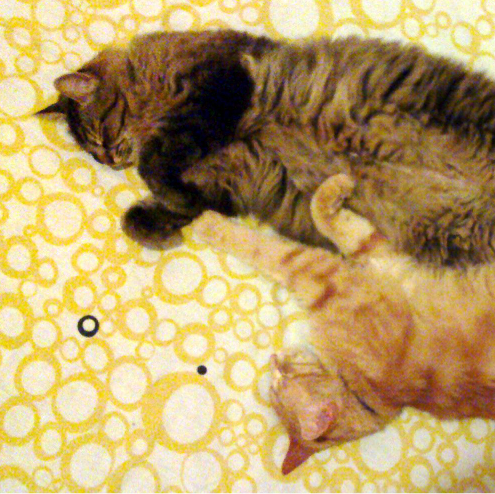
\includegraphics[width=0.2\columnwidth]{figures/cats}
  \caption{This is a sample figure}~\label{fig:figure2}
\end{figure}
\begin{itemize}
\item A
\item simple
\item list
\end{itemize}

\section{Introduction}
TODO DING\\
Introduction of problem, motivation and goals.

\section{Milestones}
TODO MARC\\
Milestones you want to reach.

\section{Equipment}
TODO ALL\\
Which equipment do you plan to utilize?

\section{Related Work}
TODO KEV\\
Overview about scientific work and existing commercial systems. How does your system compare to related work and what makes it different / better?
\subsection{Route Planning}
Investigating and Supporting Undirected Navigation for Runners \cite{undirectedrunnernav}\\
Follow the Pioneers \cite{followthepioneers} \\
Computing New Optimized Routes for GPS Navigators \cite{evolutionaryalgonav} \\
Development of a Navigation System with a Route Planning Algorithm Using Body-Worn Sensors \cite{routeplanningbodywornsensors} 
\subsection{Exploration}
Investigating and Supporting Undirected Navigation for Runners \cite{undirectedrunnernav} \\
''I Did It My Way'': Moving Away from the Tyranny of Turn-by-Turn Pedestrian Navigation \cite{ididitmyway} \\
Understanding Geocaching Practices and Motivation \cite{o2008understanding} \\
\subsection{Motivation and Design}
Sightseeing Tourists Motivation and Satisfaction \cite{DUNNROSS1991226} \\
Analysis of Intrinsic and Extrinsic Motivation in Sport \cite{vallerand1999integrative} \\
Understanding Geocaching Practices and Motivation \cite{o2008understanding} \\


\section{Evaluation \& Testing}
TODO LUKAS\\
How do you plan to test and evaluate your system?


% BALANCE COLUMNS
\balance{}

% REFERENCES FORMAT
% References must be the same font size as other body text.
\bibliographystyle{SIGCHI-Reference-Format}
\bibliography{sample}

\end{document}

%%% Local Variables:
%%% mode: latex
%%% TeX-master: t
%%% End:
